\section{Unequal precision}

\begin{frame}{How precisely can we predict demand?}
    In Lecture 07 we studied 53 customers of an electric utility. How does maximum demand (kW) vary with electricity usage (kWh)?
    \begin{center}
        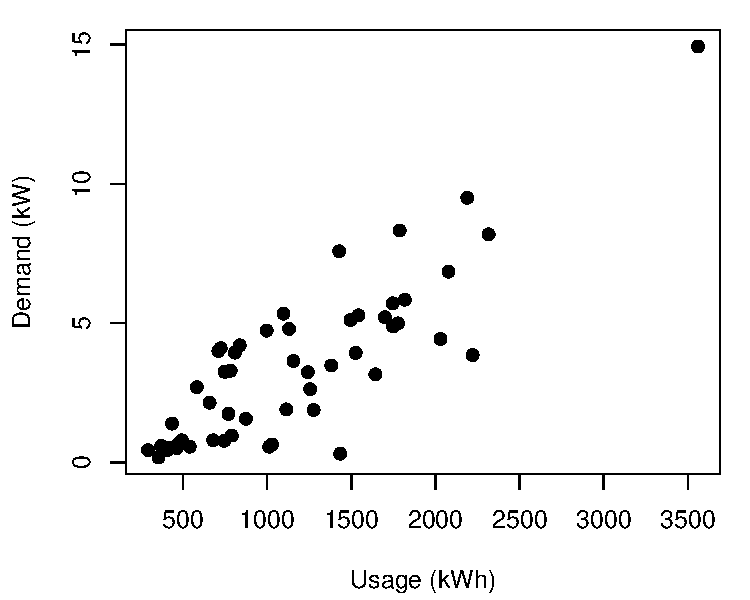
\includegraphics[width=.58\linewidth,height=.49\textheight,keepaspectratio]{../07_transformation-of-variables/figures/eu_scatter.pdf}
    \end{center}
    Compare customers near 500 kWh with those near 1500 kWh. Look separately at the average demand and the vertical spread.
\end{frame}

\begin{frame}{Read the residuals before choosing a remedy}
    \begin{center}
        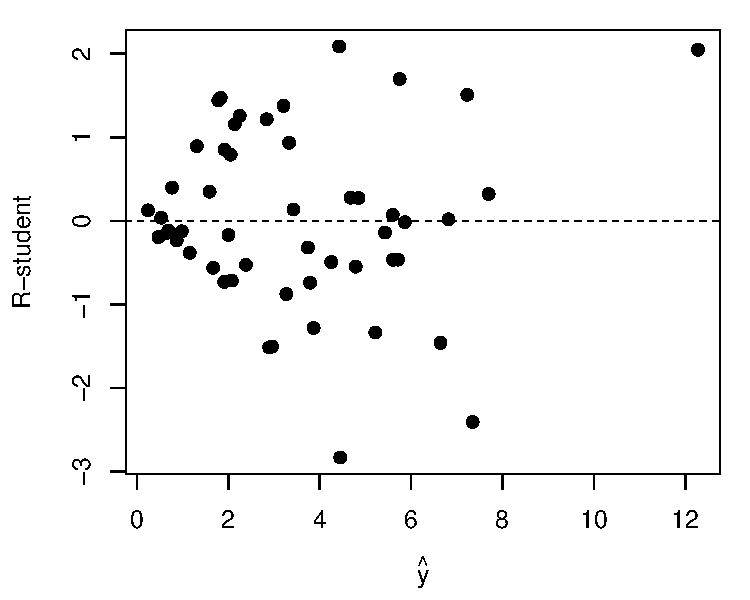
\includegraphics[width=.60\linewidth,height=.56\textheight,keepaspectratio]{../07_transformation-of-variables/figures/eu_rstudent_original.pdf}
    \end{center}
    Residuals at low fitted demand cluster near zero. Farther right, customers with similar fitted demand can have quite different observed demands.
\end{frame}

\begin{frame}{Keep the response in kilowatts}
    Lecture 07 fitted a straight line to $\sqrt{Y}$. Its fitted value estimates $\E(\sqrt{Y}\mid x)$. Squaring it requires care:
    \[
        \E(Y\mid x)=\{\E(\sqrt{Y}\mid x)\}^2+\Var(\sqrt{Y}\mid x).
    \]
    Today we model $\E(Y\mid x)=\beta_0+\beta_1x$ directly. We allow the error variance to depend on usage. How much should each customer contribute to estimating that line?
\end{frame}

\begin{frame}{Two instruments measure the same quantity}
    Independent instruments both measure a common mean $\mu$ without bias.
    \begin{center}
        \begin{tabular}{lrr}
            \toprule & Reading & Known SD \\ \midrule
            Instrument 1 & 10 & 1 \\
            Instrument 2 & 16 & 3 \\ \bottomrule
        \end{tabular}
    \end{center}
    The ordinary mean is 13. Consider $aY_1+(1-a)Y_2$. Every choice of $a$ gives an unbiased estimate. Which choice has the smallest variance?
\end{frame}

\begin{frame}{Choose the weights by minimizing variance}
    Independence gives
    \[
        V(a)=a^2+9(1-a)^2,\qquad V'(a)=2a-18(1-a).
    \]
    Setting the derivative to zero gives $a=0.9$. The estimate is $0.9(10)+0.1(16)=10.6$.
    \begin{itemize}
        \item Its variance is $0.9^2+9(0.1)^2=0.9$. The ordinary mean has variance $(1+9)/4=2.5$.
        \item The ratio $9:1$ equals the ratio of precisions $1/1^2:1/3^2$. Precision is the reciprocal of variance.
    \end{itemize}
\end{frame}

\begin{frame}{The same estimate minimizes a weighted loss}
    \[
        Q(m)=(10-m)^2+(16-m)^2/9.
    \]
    \begin{center}
        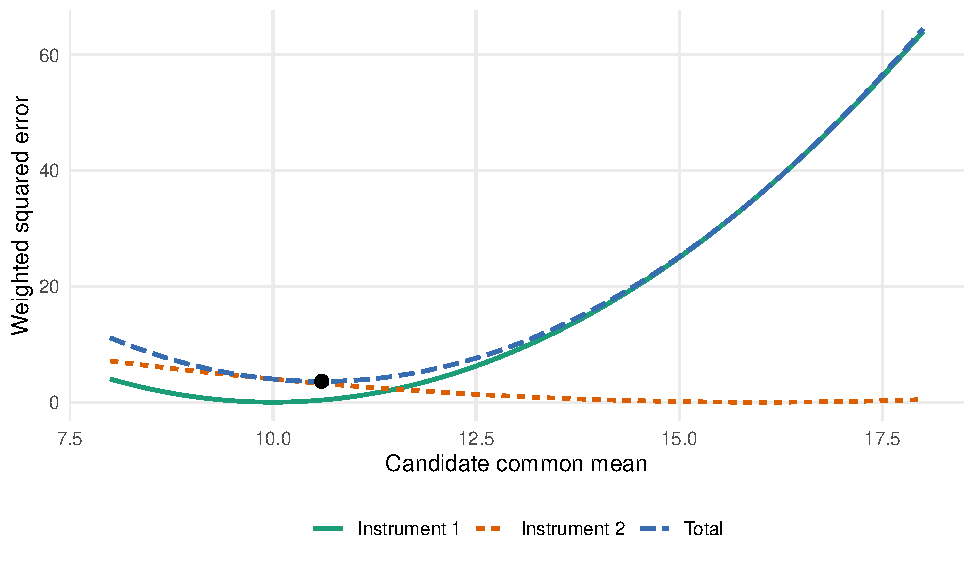
\includegraphics[width=.66\linewidth,height=.48\textheight,keepaspectratio]{figures/precision-loss.pdf}
    \end{center}
    The dot marks $Q(10.6)=3.6$. Missing the second reading by 3 units costs as much as missing the first by 1.
\end{frame}

\section{The weighted regression model}

\begin{frame}{From a common mean to a regression line}
    For observation $i$, let $\bx_i^T$ denote row $i$ of a full-rank design matrix with $p$ columns, including the intercept. Assume independent errors with
    \[
        Y_i=\bx_i^T\bbeta+\varepsilon_i,\quad
        \E(\varepsilon_i\mid\bX)=0,\quad
        \Var(\varepsilon_i\mid\bX)=\sigma^2/w_i,\quad w_i>0.
    \]
    Weighted least squares (WLS) chooses $\bb$ to minimize
    \[
        Q(\bb)=\sum_{i=1}^n w_i(y_i-\bx_i^T\bb)^2.
    \]
    Equal weights give ordinary least squares (OLS).
\end{frame}

\begin{frame}{What happens to OLS under unequal variances?}
    With $\bA=(\bX^T\bX)^{-1}\bX^T$ and $\bW=\mathrm{diag}(w_1,\ldots,w_n)$,
    \[
        \hat{\bbeta}_{O}=\bbeta+\bA\bvarepsilon,\qquad
        \Var(\hat{\bbeta}_{O}\mid\bX)=\sigma^2\bA\bW^{-1}\bA^T.
    \]
    \begin{itemize}
        \item The zero conditional error mean still gives unbiased coefficients.
        \item The familiar OLS covariance $\sigma^2(\bX^T\bX)^{-1}$ assumes equal error variances with weights normalized to one.
        \item If the relative variances are known, we can use them to estimate the coefficients more efficiently.
    \end{itemize}
\end{frame}

\begin{frame}{Transform one observation by hand}
    Multiply both sides of each equation by $\sqrt{w_i}$. For a straight line:
    \begin{center}
        \begin{tabular}{rrrr}
            \toprule $x_i$ & $w_i$ & Transformed response & Transformed design row \\ \midrule
            5 & 4 & $2y_i$ & $(2,10)$ \\
            8 & 1 & $y_i$ & $(1,8)$ \\ \bottomrule
        \end{tabular}
    \end{center}
    The first transformed column is $\sqrt{w_i}$. When fitting these transformed rows in software, supply that column explicitly and suppress the automatic intercept.
\end{frame}

\begin{frame}{The transformed errors have equal variance}
    Let $\by^*=\bW^{1/2}\by$ and $\bX^*=\bW^{1/2}\bX$. Then
    \[
        \by^*=\bX^*\bbeta+\bvarepsilon^*,\qquad
        \Var(\bvarepsilon^*\mid\bX)
        =\bW^{1/2}(\sigma^2\bW^{-1})\bW^{1/2}=\sigma^2\bI.
    \]
    The transformed residual sum of squares is exactly $Q(\bb)$. Lecture 04's Gauss--Markov result now applies: with correct fixed relative weights, WLS has minimum covariance among linear unbiased estimators.
\end{frame}

\begin{frame}{The weighted normal equations}
    Differentiating the weighted criterion gives
    \[
        -2\bX^T\bW(\by-\bX\bb)=\bzero
        \quad\Longrightarrow\quad
        \hat{\bbeta}_{W}=(\bX^T\bW\bX)^{-1}\bX^T\bW\by.
    \]
    \begin{itemize}
        \item The first normal equation for a model with an intercept is $\sum_i w_i e_i=0$, where $e_i=y_i-\hat y_i$.
        \item For an intercept-only model, $\hat\beta_0=\sum_i w_i y_i/\sum_i w_i$. This recovers 10.6 in the instrument example.
    \end{itemize}
\end{frame}

\begin{frame}{Standard errors and confidence intervals}
    Applying OLS results to $\bX^*$ gives
    \[
        \Var(\hat{\bbeta}_W\mid\bX)=\sigma^2(\bX^T\bW\bX)^{-1},
        \qquad s_W^2=\frac{\sum_i w_i e_i^2}{n-p}.
    \]
    Replace $\sigma^2$ by $s_W^2$ and take square roots of diagonal entries to obtain standard errors. With independent normal errors and known relative weights, an exact $100(1-\alpha)\%$ interval for $\beta_j$ is
    \[
        \hat\beta_{W,j}\ \pm\ t_{1-\alpha/2,n-p}\,\se(\hat\beta_{W,j}).
    \]
\end{frame}

\begin{frame}{Does multiplying every weight by 100 matter?}
    \begin{itemize}
        \item $Q(\bb)$ becomes $100Q(\bb)$. Its minimum occurs at the same coefficient vector.
        \item The estimated scale $s_W^2$ increases by a factor of 100.
        \item The inverse information matrix $(\bX^T\bW\bX)^{-1}$ decreases by a factor of 100.
    \end{itemize}
    Their product, the estimated coefficient covariance, stays the same. We can normalize the smallest weight to 1 when reporting relative weights.
\end{frame}

\begin{frame}{How much precision can correct weights buy?}
    Imagine measuring responses at 50 equally spaced values of $x$ from 1 to 10:
    \[
        Y_i=2+3x_i+x_i Z_i,\qquad Z_i\ \text{independent standard normal}.
    \]
    \begin{enumerate}
        \item Hold the design fixed and draw a new set of 50 errors.
        \item Fit OLS and WLS to the same responses, using $w_i=1/x_i^2$ for WLS.
        \item Record both slopes. Repeat 5000 times.
    \end{enumerate}
    Before seeing the results: where should each distribution be centered? Which one should be narrower?
\end{frame}

\begin{frame}{The same true slope, estimated 5000 times}
    \begin{center}
        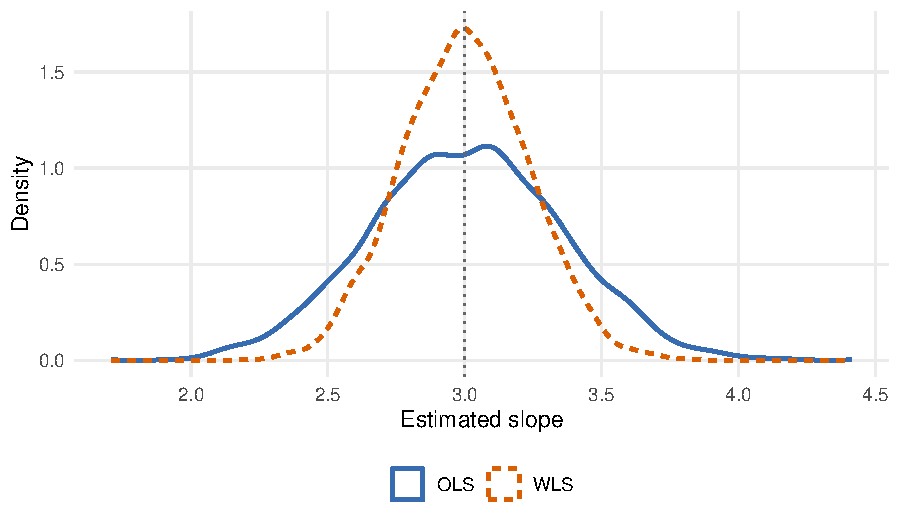
\includegraphics[height=.54\textheight,width=.75\linewidth,keepaspectratio]{figures/slope-simulation.pdf}
    \end{center}
    The dotted line marks the true slope of 3. The mean slopes were 3.007 for OLS and 3.002 for WLS. The visible difference is in their sampling spread.
\end{frame}

\begin{frame}{Compare sampling variation with the theory}
    \begin{center}
        \begin{tabular}{lrr}
            \toprule & Empirical SD of slopes & Exact SD at this design \\ \midrule
            OLS & 0.350 & 0.349 \\
            WLS & 0.232 & 0.233 \\ \bottomrule
        \end{tabular}
    \end{center}
    Correct weighting reduces the slope's sampling SD by about one third. The empirical SD measures variation \emph{across datasets}. A model-based SE estimates uncertainty from \emph{one dataset}.
    \mode<article>{To reproduce the exact column, write each fitted slope as $\sum_i a_iY_i$, with $a_i$ taken from the slope row of the appropriate least-squares coefficient matrix. At this fixed design, independence gives $\Var(\sum_i a_iY_i)=\sum_i a_i^2 x_i^2$. The simulation can therefore be checked without relying on either model's reported standard errors.}
\end{frame}
\section{Estimating weights for utility customers}

\begin{frame}{First fit the demand model by OLS}
    Using all 53 customers, with $x$ in kWh and $y$ in kW,
    \[
        \hat y_O=-0.83130+0.00368284x.
    \]
    An additional 100 kWh corresponds to an estimated 0.3683 kW increase in mean demand. The intercept describes zero usage, outside the observed range of 292 to 3560 kWh.
    \svspace{0.5em}

    Keep the raw residuals $e_{O,i}=y_i-\hat y_{O,i}$. They supply information about how the scatter changes with usage.
\end{frame}

\begin{frame}{Where can precision weights come from?}
    \begin{itemize}
        \item \textbf{Calibration.} If the measuring instrument has known variance $v_i$, use $w_i\propto 1/v_i$.
        \item \textbf{Replicate means.} If $y_i$ averages $m_i$ independent readings, each with variance $\sigma^2$, its variance is $\sigma^2/m_i$. Use $w_i=m_i$.
        \item \textbf{Estimated spread.} With one demand measurement per customer, pool information across customers by modeling error spread as a function of usage.
    \end{itemize}
    Customer weights in this example describe precision of demand observations.
\end{frame}

\begin{frame}{Fit a working model for the error spread}
    Suppose $\varepsilon_i=c x_i^\gamma Z_i$, where $c>0$, $x_i>0$ and the standardized errors share a distribution. Then
    \[
        \log|\varepsilon_i|=\log c+\gamma\log x_i+\log|Z_i|.
    \]
    Use $\log|e_{O,i}|$ as the response in an auxiliary regression on $\log x_i$. The intercept absorbs the mean of $\log|Z_i|$.
    \svspace{0.5em}

    This is an approximation: residuals depend on the fitted line and on leverage. Check for zero residuals before taking logarithms.
\end{frame}

\begin{frame}{How strong is the spread trend?}
    \begin{center}
        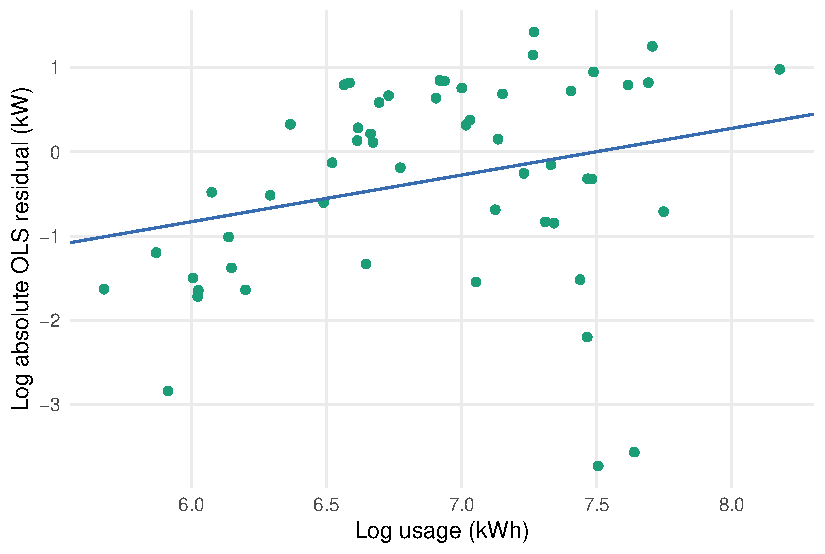
\includegraphics[width=.65\linewidth,height=.52\textheight,keepaspectratio]{figures/utility-spread.pdf}
    \end{center}
    Estimated slope $0.554$ (SE $0.277$), $R^2=0.073$. The positive trend suggests trying $w_i\propto x_i^{-2(0.554)}$. The wide scatter makes a residual check especially important.
\end{frame}

\begin{frame}{Apply the estimated weights and refit}
    Normalize the weights as $w_i=(x_i/3560)^{-1.10805}$. The customer at 292 kWh receives about 16 times the weight of the customer at 3560 kWh.
    \begin{center}
        \begin{tabular}{lrr}
            \toprule & OLS (SE) & WLS (SE) \\ \midrule
            Intercept (kW) & $-0.8313\ (0.4416)$ & $-0.6646\ (0.3276)$ \\
            Slope per 100 kWh & $0.3683\ (0.0334)$ & $0.3538\ (0.0347)$ \\
            \bottomrule
        \end{tabular}
    \end{center}
    Weighting changes the slope modestly. Its reported model-based SE increases slightly. The WLS calculation treats the fitted weights as fixed.
\end{frame}

\begin{frame}{How far apart are the fitted means?}
    \begin{center}
        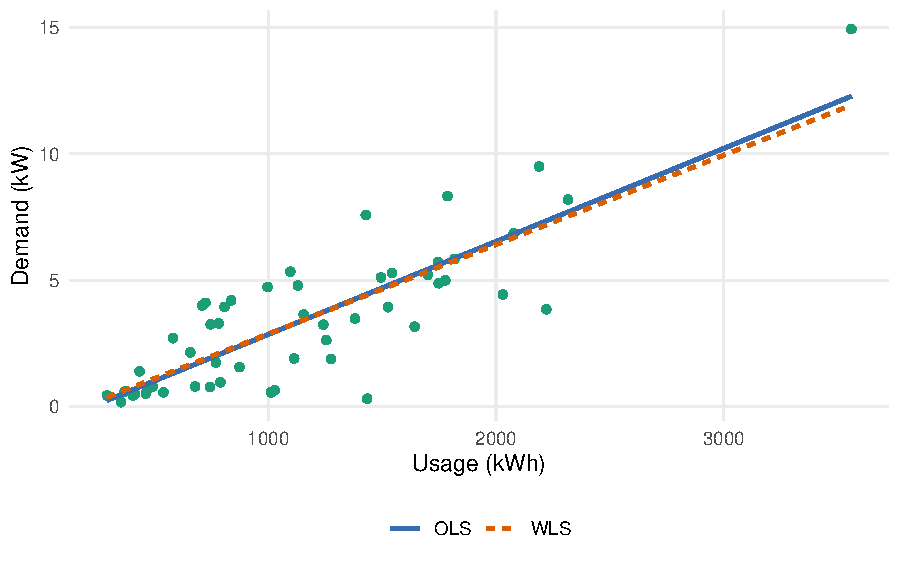
\includegraphics[width=.72\linewidth,height=.52\textheight,keepaspectratio]{figures/utility-fits.pdf}
    \end{center}
    At 1000 kWh, the fitted mean demand is 2.852 kW under OLS and 2.873 kW under WLS. Their model-based 95\% intervals for the mean are $(2.405,3.298)$ and $(2.497,3.249)$ kW, respectively.
\end{frame}

\begin{frame}{Feasible weighted least squares}
    We estimated the variance pattern and then inserted those estimates into the weighted fit. This two-stage procedure is called \emph{feasible WLS}.
    \begin{itemize}
        \item Misspecifying the mean can create apparent changes in residual size. Check the fitted mean before interpreting a variance trend.
        \item Weight estimation adds uncertainty. The fixed-weight $t$ argument alone cannot establish exact coverage for these intervals.
    \end{itemize}
    \mode<article>{For independent sampled customers, a pairs bootstrap can repeat the entire calculation: resample customer records, refit OLS, re-estimate the spread exponent and refit WLS. The resulting distribution of slopes reflects variation in both fitted stages.}
\end{frame}

\section{Checking the weighted fit}

\begin{frame}{Which residual should we plot?}
    Raw residuals $e_i=y_i-\hat y_i$ measure prediction errors in kW. To check the working variance model, use the transformed residuals
    \[
        e_i^*=\sqrt{w_i}(y_i-\hat y_i).
    \]
    Customer 2 used 292 kWh and had demand 0.44 kW. Its WLS prediction is 0.3684 kW. With $w_2=15.974$, its transformed residual is
    \[
        \sqrt{15.974}(0.44-0.3684)\approx 0.286.
    \]
\end{frame}

\begin{frame}{Allow for leverage in the transformed design}
    Let $h^*_{ii}$ be diagonal element $i$ of the hat matrix for $\bX^*$. Under the assumed variance model,
    \[
        \Var(e_i^*\mid\bX)=\sigma^2(1-h^*_{ii}),\qquad
        r_i^*=\frac{\sqrt{w_i}\,e_i}{s_W\sqrt{1-h^*_{ii}}}.
    \]
    For customer 2, $h^*_{22}=0.119$ and $s_W=2.870$. Its standardized residual is about $0.11$. A large precision weight can accompany a small standardized residual.
\end{frame}

\begin{frame}{Did weighting stabilize the spread?}
    \begin{center}
        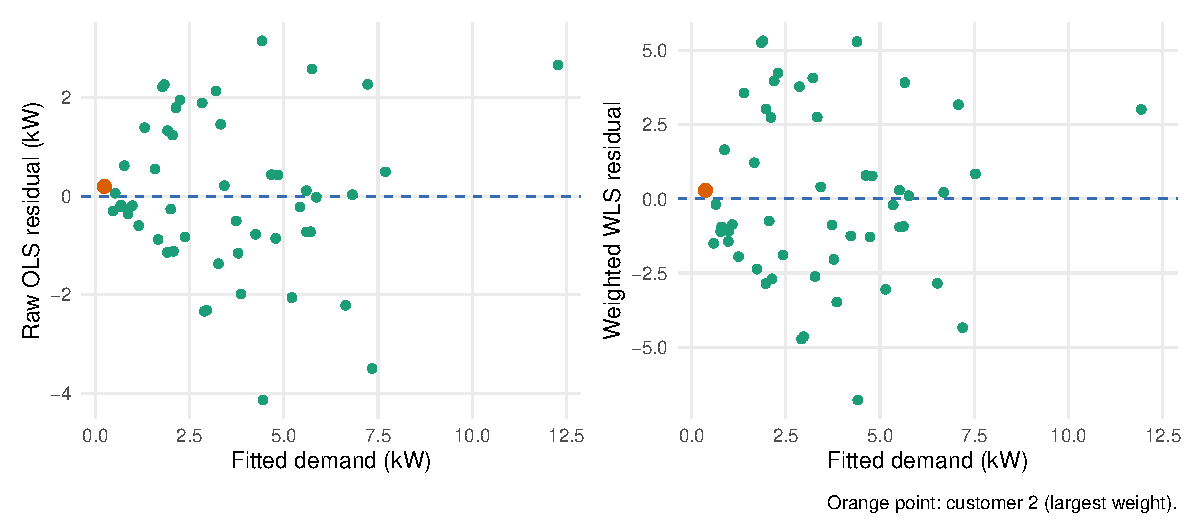
\includegraphics[width=.90\linewidth,height=.50\textheight,keepaspectratio]{figures/utility-residuals.pdf}
    \end{center}
    From lowest to highest usage quartile, raw OLS residual SDs are 0.57, 1.74, 1.88 and 1.86. After weighting they are 1.60, 3.82, 3.23 and 2.47 on the transformed scale. The lowest-usage group still has the smallest spread.
\end{frame}

\begin{frame}{Does estimating the exponent change the conclusion?}
    The fitted variance exponent is 1.108. Try the simpler working assumption $\Var(Y_i\mid x_i)\propto x_i$, giving $w_i\propto1/x_i$.
    \begin{center}
        \begin{tabular}{lrr}
            \toprule Weight rule & Slope per 100 kWh & Model-based SE \\ \midrule
            Equal & 0.36828 & 0.03339 \\
            $1/x_i$ & 0.35379 & 0.03447 \\
            $1/x_i^{1.108}$ & 0.35376 & 0.03471 \\ \bottomrule
        \end{tabular}
    \end{center}
    Rounding the exponent to one changes the estimated increase in mean demand by only 0.00003 kW per 100 kWh.
\end{frame}

\begin{frame}{Which weight rule makes the spread most even?}
    Split customers into four groups by usage. Within each group, compute the SD of the fit's internally standardized residuals.
    \begin{center}
        \begin{tabular}{lrrrr}
            \toprule Weight rule & Lowest & Second & Third & Highest \\ \midrule
            Equal & 0.37 & 1.12 & 1.20 & 1.25 \\
            $1/x_i$ & 0.55 & 1.33 & 1.15 & 0.92 \\
            $1/x_i^{1.108}$ & 0.57 & 1.34 & 1.14 & 0.89 \\ \bottomrule
        \end{tabular}
    \end{center}
    Both weighting rules reduce the discrepancy between the lowest and highest groups. The second group still has more than twice the spread of the first. Each group contains only about 13 customers.
\end{frame}

\begin{frame}{What would we report to the utility?}
    \begin{itemize}
        \item \textbf{Mean demand.} The estimated increase per 100 kWh is about 0.35--0.37 kW across all three fits. The substantive slope conclusion is stable.
        \item \textbf{Working weights.} For a weighted analysis, use the simpler inverse-usage rule and show OLS as a sensitivity check. Estimating an extra exponent adds little here.
        \item \textbf{Individual predictions.} Both weighted fits leave substantial differences in spread across usage groups. Check interval coverage with additional customers before relying on nominal 95\% coverage for a particular usage group.
    \end{itemize}
\end{frame}
\begin{frame}{Predicting one new customer's demand}
    For a new predictor row $\bx_0^T$, the variance of the estimated mean uses
    $v_0=\bx_0^T(\bX^T\bW\bX)^{-1}\bx_0$:
    \[
        \widehat{\se}(\hat y_0)=s_W\sqrt{v_0},\qquad
        \widehat{\se}(Y_0-\hat y_0)=s_W\sqrt{v_0+1/w_0}.
    \]
    The second expression assumes an independent new error with variance $\sigma^2/w_0$. For a utility customer we must assign $w_0$ from the fitted usage rule using the same normalization as in training.
\end{frame}

\begin{frame}{At 1000 kWh, how uncertain is one new demand?}
    Continue with the estimated-power fit so we can use its reported scale. For a customer using 1000 kWh,
    \[
        w_0=(1000/3560)^{-1.10805}=4.084,\qquad s_W=2.870.
    \]
    The fitted mean has SE 0.1875 kW. An independent new demand has an additional error variance estimated by $2.870^2/4.084$. Hence
    \[
        \widehat{\se}(Y_0-\hat y_0)
        =\sqrt{0.1875^2+2.870^2/4.084}=1.433\ \mathrm{kW}.
    \]
\end{frame}

\begin{frame}{Same fitted value, two different intervals}
    At 1000 kWh, the fitted mean demand is 2.873 kW. Using $t_{0.975,51}=2.008$:
    \begin{center}
        \begin{tabular}{lrr}
            \toprule Target & SE (kW) & Model-based 95\% interval (kW) \\ \midrule
            Mean demand & 0.1875 & $(2.497,\ 3.249)$ \\
            One new customer & 1.4325 & $(-0.003,\ 5.749)$ \\ \bottomrule
        \end{tabular}
    \end{center}
    The slightly negative lower limit is physically impossible. It comes from a symmetric error model on the original scale. Treat the interval as approximate and examine the lower tail when individual forecasts matter.
\end{frame}
\begin{frame}{Practice: choose the weights}
    Give relative weights for each observation and identify the transformed residual.
    \begin{enumerate}
        \item Error SD is proportional to a positive predictor $x_i$.
        \item Error variance is proportional to $x_i$.
        \item The response is the mean of $m_i$ equally precise independent measurements.
    \end{enumerate}
    \pause
    \begin{center}
        \begin{tabular}{lcc}
            \toprule & Relative weight & Transformed residual \\ \midrule
            1 & $1/x_i^2$ & $e_i/x_i$ \\
            2 & $1/x_i$ & $e_i/\sqrt{x_i}$ \\
            3 & $m_i$ & $\sqrt{m_i}\,e_i$ \\ \bottomrule
        \end{tabular}
    \end{center}
\end{frame}

\begin{frame}{A curved center after weighting}
    Suppose the weighted residuals have similar vertical spread throughout, but their average follows a U-shaped curve across fitted values. What should change?
    \pause
    \begin{itemize}
        \item The spread check supports the working variance pattern. The curved center points to a problem with the fitted mean.
        \item Revisit the predictors and the shape of $\E(Y\mid x)$. Weighting changes the contribution of observations to the fitted line; a straight-line mean still forces a constant slope.
        \item In Lecture 14 we allow the slope to vary with wind speed and compare polynomial and nonlinear mean curves.
    \end{itemize}
\end{frame}
